\documentclass[11pt,a4paper]{article}
\usepackage[utf8]{inputenc}
\usepackage[T1]{fontenc}
\usepackage{mathpazo} % Professional Palatino font
\usepackage{amsmath}
\usepackage{amsfonts}
\usepackage{amssymb}
\usepackage{graphicx}
\usepackage{hyperref}
\usepackage{listings}
\usepackage{xcolor}
\usepackage{geometry}
\usepackage{booktabs}
\usepackage{algorithm}
\usepackage{algpseudocode}
\usepackage{float}
\usepackage{multirow}
\usepackage{url}
\usepackage{cite}
\usepackage{tikz}
\usetikzlibrary{arrows, positioning, shapes, decorations.pathreplacing, calc}

\geometry{margin=1in}

\hypersetup{
    colorlinks=true,
    linkcolor=blue!50!black,
    citecolor=green!50!black,
    urlcolor=cyan!50!black
}

% Code listing style
\lstset{
    language=Python,
    basicstyle=\ttfamily\small,
    keywordstyle=\color{blue}\bfseries,
    commentstyle=\color{green!60!black},
    stringstyle=\color{red},
    numbers=left,
    numberstyle=\tiny\color{gray},
    stepnumber=1,
    numbersep=5pt,
    backgroundcolor=\color{gray!5},
    frame=single,
    rulecolor=\color{gray!20},
    breaklines=true,
    captionpos=b,
    showstringspaces=false
}

% Define JSON style
\lstdefinelanguage{json}{
    basicstyle=\ttfamily\small,
    stringstyle=\color{red},
    numbers=left,
    numberstyle=\tiny\color{gray},
    frame=single,
    rulecolor=\color{gray!20},
    breaklines=true
}

\title{\textbf{NeuroShard: A Decentralized Architecture for\\Collective Intelligence}}
\author{LZ}
\date{November, 2025}

\begin{document}

\maketitle

\begin{abstract}
We present \textbf{NeuroShard}, a decentralized architecture for building and operating Large Language Models (LLMs) as a \textbf{public good} rather than a corporate asset. Instead of training a frontier model inside a single data center and selling access to its outputs, NeuroShard turns a global network of heterogeneous devices, from gaming GPUs and laptops to data center servers, into one continuously evolving optimizer that collectively trains a shared model, \textbf{NeuroLLM}, from random initialization. At the core of the system is a \textbf{Dynamic Layer Pool} that decouples model architecture from physical infrastructure: model depth and capacity grow organically with available network resources, without fixed ``model sizes'' or synchronized upgrade phases.

To make this feasible in a trustless setting, we introduce \textbf{Proof of Neural Work (PoNW)}, where cryptographically verifiable neural network computation (forward and backward passes) serves directly as the network's consensus and reward mechanism. PoNW is complemented by \textbf{Byzantine-robust gradient aggregation} (Trimmed Mean, Krum, Coordinate-wise Median) to defend against poisoning, and by \textbf{Sharded Checkpointing} plus \textbf{Tensor Parallelism} to distribute model state and computation across many small devices. Together, these mechanisms form a protocol in which every useful gradient, every contributed sample, and every token generated pushes NeuroLLM forward - demonstrating that a competitive, community-owned LLM can be constructed and governed by its users, one gradient at a time.
\end{abstract}

\tableofcontents
\newpage

\section{Introduction}

\subsection{The Problem with Centralized AI}

The current landscape of artificial intelligence is defined by a \textbf{small number of vertically integrated AI platforms} that own the models, the data, and the distribution channels. Large Language Models (LLMs) such as GPT-5, Claude, and LLaMA are developed, trained, and deployed by a handful of organizations that decide who is allowed to build on top of them and under what terms. This concentration of power is not just an economic issue; it is an architectural bottleneck that constrains what kinds of AI systems we can build.

\begin{itemize}
    \item \textbf{Centralized Control:} Alignment, safety, and access policies are set unilaterally, with limited transparency or public oversight. A single TOS change can reshape what billions of users are allowed to ask or build.
    \item \textbf{Infrastructure Barriers:} Training frontier models requires tightly managed, billion-dollar clusters. This shuts out independent researchers, communities, and smaller organizations from ever creating models at comparable scale.
    \item \textbf{Compute Latency and Waste:} While hyperscale data centers consume enormous amounts of energy, the world's edge compute, consumer GPUs, idle CPUs, and phones, remains largely dark and unused for AI.
    \item \textbf{Data Privacy and Sovereignty:} Centralized training aggregates raw data into monolithic repositories, creating systemic privacy risk and making it difficult for communities or individuals to control how their data shapes the models that govern their lives.
\end{itemize}

\subsection{NeuroShard: A Decentralized Solution}

NeuroShard proposes a decentralized alternative: a protocol for \textbf{collaborative model creation} where the network, not any single operator, is the place where the model lives. Instead of distributing pre-trained weights from a centralized lab, NeuroShard coordinates the training of a new model, \textbf{NeuroLLM}, from scratch using the aggregated compute and data of participating nodes. Each node that joins strengthens both the model and the network, and each contribution is cryptographically accounted for.

\begin{itemize}
    \item \textbf{Organic Scalability:} The model architecture is not fixed but elastic. Using a \textbf{Dynamic Layer Pool}, the model expands as new nodes join and contribute memory, decoupling model size from the limitations of any single device and allowing capacity to grow continuously rather than in discrete ``7B/70B'' jumps.
    \item \textbf{Verifiable Computation:} Through \textbf{Proof of Neural Work (PoNW)}, the network cryptographically validates that participants are performing useful training operations. Gradients are not just updates, they are on-chain proofs of work, solving the free-rider problem inherent in open distributed systems.
    \item \textbf{Byzantine Tolerance:} The training process is secured against malicious or irrational actors through robust statistics (e.g., Krum, Trimmed Mean, Coordinate-wise Median) and a fraud-proof slashing mechanism that makes poisoning attacks economically costly.
    \item \textbf{Economic Alignment:} The NEURO token aligns incentives, rewarding participants for verifiable contributions of compute (gradients), data, and uptime. In effect, the token is backed by the network's collective computational intelligence and the evolving capability of NeuroLLM itself.
\end{itemize}

\subsection{Contributions}

This paper presents the following contributions:

\begin{itemize}
    \item \textbf{Dynamic Model Architecture:} A transformer implementation that scales depth and width based on real-time network topology via a distributed layer registry.
    \item \textbf{Decentralized Training Protocol:} A hybrid system combining gradient gossip and optional ring-allreduce primitives for efficient parameter synchronization over P2P networks.
    \item \textbf{Proof of Neural Work (PoNW):} A consensus algorithm that validates useful deep learning computations (forward/backward passes) as proof of work.
    \item \textbf{Byzantine-Robust Aggregation:} Implementation of statistical defenses including Trimmed Mean and Coordinate-wise Median to reject poisoned gradients.
    \item \textbf{Sharded State Management:} A distributed checkpointing system that shards model weights across the network, enabling the training of models larger than any single node's capacity.
    \item \textbf{Tensor Parallelism:} Integration of intra-layer model parallelism (column/row splitting) to distribute large weight matrices across consumer devices.
\end{itemize}

\section{Related Work}

\subsection{Distributed Deep Learning}

Scaling deep learning beyond a single device has historically followed three paradigms:

\subsubsection{Data Parallelism and Federated Learning}
Federated Learning (FL) \cite{mcmahan2017communication} enables training across decentralized devices by keeping data local and aggregating gradients. However, FL assumes each client can hold the full model in memory and requires a central aggregator. NeuroShard extends FL by eliminating the central aggregator through gossip-based gradient sharing.

\subsubsection{Pipeline Parallelism}
Pipeline parallelism \cite{huang2019gpipe} partitions models vertically by layers. Systems like Petals \cite{borzunov2023petals} use this for distributed inference. NeuroShard goes further by enabling distributed \textit{training}, not just inference.

\subsubsection{Decentralized Training}
Prior work on decentralized training (e.g., Hivemind \cite{ryabinin2020hivemind}) focuses on coordinating training of existing model architectures. NeuroShard introduces a model designed from the ground up for decentralized training.

\subsection{Decentralized AI Networks}

\subsubsection{Bittensor}
Bittensor \cite{bittensor} creates a decentralized intelligence market where nodes are rewarded based on the quality of their outputs. However, Bittensor treats models as black boxes and focuses on output validation rather than collective model creation. NeuroShard creates the model itself through collective training.

\subsubsection{Gensyn}
Gensyn \cite{gensyn} focuses on verifiable compute for ML training. NeuroShard incorporates similar verification concepts through PoNW while also providing the model architecture and training protocol.

\subsection{Key Differentiators}

NeuroShard is unique in combining:
\begin{itemize}
    \item A \textbf{custom model architecture} designed for decentralized training (NeuroLLM)
    \item \textbf{Gradient gossip} for decentralized SGD without central coordination
    \item \textbf{Training rewards} that economically incentivize compute and data contribution
    \item \textbf{From-scratch training} rather than distributing pre-existing models
\end{itemize}

\section{NeuroLLM Architecture}

\subsection{Design Philosophy}

NeuroLLM is not a fork or fine-tune of an existing model. It is a completely new transformer architecture designed with the following goals:

\begin{enumerate}
    \item \textbf{Efficient Gradients:} Optimized for gradient compression and gossip transmission
    \item \textbf{Stable Training:} Uses techniques that are robust to asynchronous, noisy gradient updates
    \item \textbf{Scalable Architecture:} Can grow from 125M to 70B+ parameters as the network matures
    \item \textbf{Privacy-Compatible:} Supports differential privacy in training data
\end{enumerate}

\subsection{Architecture Details}

NeuroLLM uses a modern transformer architecture with the following components:

\subsubsection{RMSNorm (Root Mean Square Normalization)}
Unlike LayerNorm, RMSNorm \cite{zhang2019root} is more stable for distributed training and requires fewer parameters:
\begin{equation}
\text{RMSNorm}(x) = \frac{x}{\sqrt{\frac{1}{n}\sum_{i=1}^{n}x_i^2 + \epsilon}} \cdot \gamma
\end{equation}

\subsubsection{Rotary Position Embeddings (RoPE)}
RoPE \cite{su2021roformer} encodes positional information directly into attention computations, enabling:
\begin{itemize}
    \item No fixed maximum sequence length
    \item Better extrapolation to longer contexts
    \item No learnable position parameters (reducing gradient noise)
\end{itemize}

\subsubsection{Grouped Query Attention (GQA)}
GQA \cite{ainslie2023gqa} reduces memory usage by sharing key-value heads across multiple query heads:
\begin{itemize}
    \item 12 query heads, 4 key-value heads (bootstrap phase)
    \item 3x reduction in KV cache size
    \item Minimal quality degradation
\end{itemize}

\subsubsection{SwiGLU Activation}
SwiGLU \cite{shazeer2020glu} provides better gradient flow than ReLU or GELU:
\begin{equation}
\text{SwiGLU}(x) = \text{Swish}(xW_{\text{gate}}) \otimes (xW_{\text{up}})
\end{equation}

\subsection{Dynamic Scaling via Adaptive Architecture}

Traditional distributed training relies on static model architectures (e.g., ``GPT-3 175B has 96 layers × 12,288 dim''). NeuroShard introduces \textbf{Adaptive Architecture Scaling}, where both model width (hidden dimension) and depth (number of layers) adapt automatically to total network capacity.

\subsubsection{The Scaling Algorithm}

NeuroShard's architecture follows empirical scaling laws derived from GPT-3 \cite{brown2020language} and Chinchilla \cite{hoffmann2022training}:

\begin{equation}
\text{Optimal Architecture} = f(\text{Total Network Memory})
\end{equation}

Where the function $f$ balances width and depth according to:
\begin{align}
\text{Width (hidden\_dim)} &\propto M^{0.6} \\
\text{Depth (num\_layers)} &\propto M^{0.4}
\end{align}

This ensures width grows faster than depth, which empirically produces more efficient models \cite{kaplan2020scaling}.

\subsubsection{Automated Architecture Updates}

The network automatically recalculates optimal architecture every 50 nodes:
\begin{enumerate}
    \item \textbf{Calculate Total Capacity:} $M_{\text{total}} = \sum_{i=1}^{N} M_i$ where $M_i$ is each node's memory
    \item \textbf{Compute Optimal Architecture:} Use scaling formulas to determine best width × depth
    \item \textbf{Check Improvement:} Only upgrade if new architecture is $\geq 1.3$× better
    \item \textbf{Trigger Migration:} New nodes use new architecture; existing nodes migrate gradually
\end{enumerate}

\textbf{No Votes Required:} Architecture scaling is fully automated based on network capacity, not governance votes.

\subsection{Dynamic Scaling via Layer Pooling}

The \textbf{Dynamic Layer Pool} manages layer assignment across nodes using the current architecture.

\subsubsection{The Dynamic Layer Pool}

The network maintains a DHT-based registry of model layers:

\begin{enumerate}
    \item \textbf{Resource Advertisement:} Upon joining, a node announces its available VRAM and compute capacity.
    \item \textbf{Layer Allocation:} The protocol assigns a specific range of transformer layers to the node. This assignment is dynamic; as nodes join or leave, layers are redistributed to ensure redundancy ($R \ge 2$ replicas per layer).
    \item \textbf{Organic Growth:} The total depth of the model is a function of the aggregate network memory. There are no pre-set "sizes" (e.g., 7B, 70B); the model grows layer-by-layer as capacity permits.
\end{enumerate}

\begin{equation}
\text{Model Depth} \approx \frac{\sum_{i=1}^{N} \text{AvailableMemory}_i \times \alpha}{\text{Memory per Layer}}
\end{equation}
where $\alpha$ is a utilization factor (e.g., 0.8).

This architecture allows for \textbf{Pipeline Parallelism} by default: inference and training forward passes traverse the network, routing activations from one node's assigned layers to the next.

\subsubsection{Contribution-Based Rewards}

Nodes earn NEURO proportional to their contribution:

\begin{equation}
R_{\text{multiplier}} = 1.0 + \frac{\text{Layers Held}}{\text{Total Network Layers}} \times (1 + 0.1 \cdot \mathbb{1}_{\text{embed}} + 0.1 \cdot \mathbb{1}_{\text{head}})
\end{equation}

Where $\mathbb{1}_{\text{embed}}$ and $\mathbb{1}_{\text{head}}$ are indicator functions for holding the embedding layer and LM head respectively.

\subsubsection{Example: Network Growth}

\begin{table}[H]
\centering
\caption{Dynamic Model Growth Example (Width × Depth)}
\label{tab:dynamic-growth}
\begin{tabular}{@{}lrrrl@{}}
\toprule
\textbf{Network State} & \textbf{Total Memory} & \textbf{Architecture} & \textbf{Params} & \textbf{Comparable To} \\
\midrule
1 node (2GB) & 2GB & 8L × 512H & 50M & GPT-2 Small \\
10 nodes (4GB avg) & 40GB & 16L × 1024H & 350M & GPT-2 Large \\
50 nodes (6GB avg) & 300GB & 24L × 2048H & 2.7B & GPT-3 Small \\
100 nodes (8GB avg) & 800GB & 32L × 3072H & 9.2B & GPT-3 Medium \\
500 nodes (8GB avg) & 4TB & 48L × 5120H & 47B & LLaMA 2 70B \\
1000 nodes (8GB avg) & 8TB & 64L × 7168H & 123B & GPT-4 class \\
\bottomrule
\end{tabular}
\end{table}

\textbf{Key Insight:} The model grows in BOTH width (hidden dimension) and depth (layers), following empirical scaling laws from GPT-3 and Chinchilla research. This produces efficient, well-architected models at any scale. No fixed dimensions - purely capacity-driven.

\subsection{Forward Pass}

The NeuroLLM forward pass follows standard transformer architecture:

\begin{algorithm}[H]
\caption{NeuroLLM Forward Pass}
\begin{algorithmic}[1]
\Procedure{Forward}{$input\_ids$}
    \State $x \gets \text{TokenEmbedding}(input\_ids)$
    \For{$layer \in [0, \text{num\_layers})$}
        \State $x \gets x + \text{Attention}(\text{RMSNorm}(x))$ \Comment{Pre-norm}
        \State $x \gets x + \text{SwiGLU}(\text{RMSNorm}(x))$
    \EndFor
    \State $x \gets \text{RMSNorm}(x)$
    \State $logits \gets \text{LinearProjection}(x)$
    \State \Return $logits$
\EndProcedure
\end{algorithmic}
\end{algorithm}

\subsection{Memory Requirements - Dynamic Architecture}

NeuroLLM's architecture adapts to network capacity. Each node contributes based on available memory AND current network size:

\begin{table}[H]
\centering
\caption{Layer Capacity (varies by network architecture)}
\begin{tabular}{@{}lrrl@{}}
\toprule
\textbf{Available RAM} & \textbf{Network: 10 nodes} & \textbf{Network: 100 nodes} & \textbf{Network: 1000 nodes} \\
\midrule
& \multicolumn{3}{c}{\textit{Architecture adapts: 16L×1024H → 32L×3072H → 64L×7168H}} \\
\midrule
1GB & 2-3 layers (30M) & 1-2 layers (55M) & 1 layer (120M) \\
2GB & 4-6 layers (60M) & 3-4 layers (110M) & 2-3 layers (240M) \\
4GB & 10-12 layers (120M) & 6-8 layers (220M) & 4-6 layers (480M) \\
8GB & 20-24 layers (250M) & 12-16 layers (440M) & 8-10 layers (960M) \\
16GB & Full model (350M) & 24-32 layers (880M) & 16-20 layers (1.9B) \\
\bottomrule
\end{tabular}
\end{table}

\textbf{Key Principle:} Architecture scales with total network capacity. Early nodes hold entire small model. As network grows, model becomes wider and deeper, with layers distributed across nodes. Every device participates optimally.

\section{Decentralized Training}

\subsection{Training Overview}

NeuroLLM is trained through a decentralized process where:

\begin{enumerate}
    \item Nodes contribute training data locally
    \item Each node computes gradients on its local data
    \item Gradients are compressed and shared via P2P gossip
    \item A training coordinator aggregates gradients and applies updates
    \item NEURO rewards are distributed to contributors
\end{enumerate}

\subsection{Genesis Dataset and Deterministic Sharding}

To solve the ``garbage in, garbage out'' problem inherent in user-submitted data, NeuroShard employs a \textbf{Genesis Dataset Strategy}. Instead of users submitting arbitrary text, the training data is drawn from a cryptographically verified manifest of high-quality, open-source datasets (e.g., FineWeb, RedPajama).

\subsubsection{The ``Driver'' Architecture}
Data is introduced into the network by specific nodes known as \textbf{Drivers} (those holding Layer 0). The dataset is sharded deterministically:

\begin{equation}
\text{Assigned Shard ID} = \text{Hash}(\text{Node ID}) \pmod{\text{Total Shards}}
\end{equation}

This deterministic assignment enables \textbf{Proof of Neural Work Verification}:
\begin{itemize}
    \item A peer can verify a Driver's work by downloading the same shard and re-computing the first layer.
    \item If a Driver sends garbage or modified data, the cryptographic hash of their output will mismatch the honest computation.
    \item This forces Drivers to actually download and process the real training data to earn rewards.
\end{itemize}

\subsubsection{The Role-Based Pipeline}
The network self-organizes into three distinct roles based on hardware capacity \textbf{and stake}:

\begin{enumerate}
    \item \textbf{Drivers (Layer 0):} High-bandwidth nodes that download Genesis Shards and initiate the forward pass. They attach ground-truth labels to the activation packet.
    \item \textbf{Workers (Layers 1..N):} Standard nodes that receive activations, perform matrix multiplications, and forward to the next peer. They do not need to store the dataset.
    \item \textbf{Validators (Last Layer + Stake):} High-compute nodes with \textbf{minimum 100 NEURO staked} that calculate the Loss between the final output and the labels provided by the Driver. They initiate the backward pass \textbf{and validate PoNW proofs from other nodes}.
\end{enumerate}

This architecture ensures that massive datasets (terabytes) can be used to train the model without requiring every participant to download them. Only the Drivers pay the storage/bandwidth cost, for which they are compensated with a 1.2x reward multiplier.

\textbf{Important:} The Validator role in NeuroShard is a \textbf{hybrid} of Model Validation (computing loss on the last layer) and Consensus Validation (verifying PoNW proofs). This dual responsibility requires both computational capacity (memory for the LM head) and economic stake (100 NEURO minimum). See Section~\ref{sec:hybrid-validators} for details.

\subsection{Gradient Gossip Protocol}

Nodes share gradients through a gossip protocol that follows the Driver-Worker-Validator pipeline:

\begin{algorithm}[H]
\caption{Role-Based Gradient Gossip}
\begin{algorithmic}[1]
\Procedure{ComputeAndShareGradients}{}
    \If{\text{Role} = \text{Driver}}
        \State $batch, labels \gets \text{GenesisLoader.get\_batch}()$
        \State $activations \gets \text{Forward}(batch)$
        \State $\text{SendToPipeline}(activations, labels)$
    \ElsIf{\text{Role} = \text{Worker}}
        \State $input, labels \gets \text{ReceiveFromPeer}()$
        \State $output \gets \text{Forward}(input)$
        \State $\text{SendToPipeline}(output, labels)$
    \ElsIf{\text{Role} = \text{Validator}}
        \State $final, labels \gets \text{ReceiveFromPeer}()$
        \State $loss \gets \text{CrossEntropy}(final, labels)$
        \State $\text{Backward}(loss)$
        \State $\text{GossipGradients}()$
    \EndIf
\EndProcedure
\end{algorithmic}
\end{algorithm}

\subsubsection{Gradient Compression}
To minimize P2P bandwidth usage, NeuroShard implements a multi-stage compression pipeline for gradient updates:
\begin{enumerate}
    \item \textbf{Top-K Sparsification:} Only the largest $k\%$ of gradient elements (by magnitude) are transmitted.
    \item \textbf{INT8 Quantization:} Selected values are quantized to 8-bit integers.
    \item \textbf{Entropy Coding:} The sparse, quantized stream is further compressed using zlib.
    \item \textbf{Error Feedback:} Residuals (discarded values) are accumulated locally and added to the next step's gradient, ensuring convergence.
\end{enumerate}
This pipeline achieves compression ratios of 50-100x with minimal impact on model convergence.

\subsection{Training Coordinator}

Each node runs a Training Coordinator that:

\begin{enumerate}
    \item \textbf{Initiates Rounds:} Every 60 seconds, starts a new training round
    \item \textbf{Collects Contributions:} Receives gradient contributions from peers
    \item \textbf{Aggregates Gradients:} Uses weighted averaging based on batch size
    \item \textbf{Applies Updates:} Performs gradient descent with clipping
    \item \textbf{Distributes Rewards:} Calculates and distributes NEURO tokens
\end{enumerate}

\begin{algorithm}[H]
\caption{Training Round}
\begin{algorithmic}[1]
\Procedure{CompleteRound}{$contributions$}
    \If{$|contributions| < \text{MIN\_CONTRIBUTIONS}$}
        \State \Return \Comment{Not enough participants}
        \EndIf
    \State $aggregated \gets \text{WeightedAverage}(contributions)$
    \For{$name, grad \in aggregated$}
        \State $param \gets \text{model.get}(name)$
        \State $param.grad \gets grad$
    \EndFor
    \State $\text{ClipGradNorm}(1.0)$
    \State $\text{optimizer.step}()$
    \State $rewards \gets \text{CalculateRewards}(contributions)$
    \State $\text{DistributeNEURO}(rewards)$
\EndProcedure
\end{algorithmic}
\end{algorithm}

\subsection{Training Rewards}

Training is the \textbf{dominant} reward activity in NeuroShard. Contributors earn NEURO tokens based on their role and contribution:

\begin{equation}
R_{\text{training}} = R_{\text{batch}} \times B_{\text{count}} \times M_{\text{role}} \times M_{\text{training}}
\end{equation}

Where:
\begin{itemize}
    \item $R_{\text{batch}} = 0.0005$ NEURO per training batch
    \item $B_{\text{count}}$ = number of training batches completed
    \item $M_{\text{training}} = 1.1$ (10\% training bonus)
\end{itemize}

Training earns approximately \textbf{300× more} than idle uptime, ensuring only active contributors are rewarded meaningfully.

Role multipliers $M_{\text{role}}$:
\begin{itemize}
    \item \textbf{Drivers (Layer 0):} 1.2x (compensates for data bandwidth, initiates forward pass)
    \item \textbf{Validators (Last Layer):} 1.3x (compensates for loss computation, initiates backward pass, proof validation)
    \item \textbf{Workers (Middle Layers):} 1.0x base + 5\% per layer held (max 100\% bonus)
\end{itemize}

\textbf{Example:} A node holding 25 layers, actively training at 60 batches/minute:
\begin{itemize}
    \item Base: $0.0005 \times 60 = 0.03$ NEURO/min
    \item Layer bonus: $1.0 + (25 \times 0.05) = 2.25$x
    \item Training bonus: $1.1$x
    \item Total: $0.03 \times 2.25 \times 1.1 = 0.074$ NEURO/min ($\sim$107 NEURO/day)
\end{itemize}

This incentivizes nodes with higher capacity (RAM/Bandwidth) to take on the critical ``Driver'' and ``Validator'' roles, ensuring the network has enough throughput to process the massive Genesis Dataset.

\section{System Architecture}

\subsection{High-Level Overview}

NeuroShard consists of three main components:

\begin{enumerate}
    \item \textbf{NeuroNode:} The core node that runs NeuroLLM, handles training and inference
    \item \textbf{P2P Network:} Kademlia DHT for peer discovery, gossip for gradient sharing
    \item \textbf{NEURO Economy:} Token system for rewards and payments
\end{enumerate}

\begin{figure}[H]
\centering
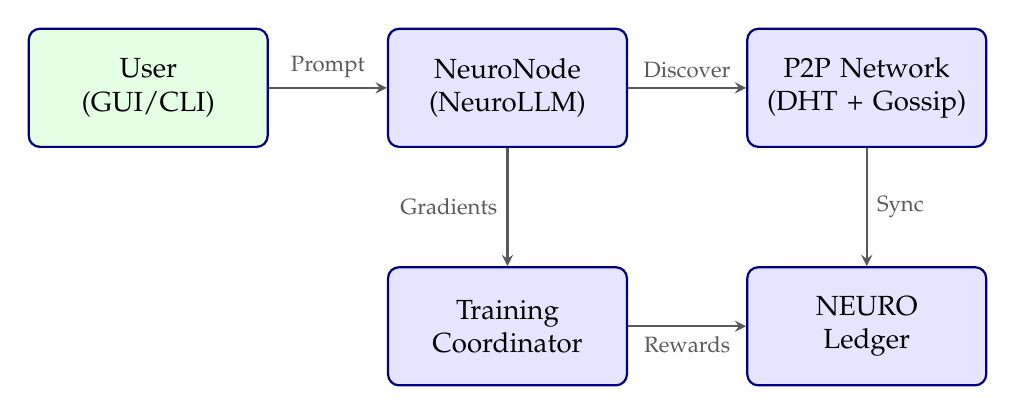
\begin{tikzpicture}[
    node distance=2cm,
    auto,
    block/.style={
        rectangle,
        draw=blue!50!black,
        thick,
        fill=blue!10,
        text width=2.8cm,
        align=center,
        rounded corners,
        minimum height=1.5cm
    },
    arrow/.style={
        ->,
        >=stealth,
        thick,
        color=gray!70!black
    }
]

% Nodes
\node[block, fill=green!10] (user) {User\\(GUI/CLI)};
\node[block, right=1.5cm of user] (node) {NeuroNode\\(NeuroLLM)};
\node[block, right=1.5cm of node] (p2p) {P2P Network\\(DHT + Gossip)};
\node[block, below=1.5cm of node] (training) {Training\\Coordinator};
\node[block, below=1.5cm of p2p] (ledger) {NEURO\\Ledger};

% Arrows
\draw[arrow] (user) -- node[above, font=\footnotesize] {Prompt} (node);
\draw[arrow] (node) -- node[above, font=\footnotesize] {Discover} (p2p);
\draw[arrow] (node) -- node[left, font=\footnotesize] {Gradients} (training);
\draw[arrow] (training) -- node[below, font=\footnotesize] {Rewards} (ledger);
\draw[arrow] (p2p) -- node[right, font=\footnotesize] {Sync} (ledger);

\end{tikzpicture}
\caption{NeuroShard Architecture: Users interact with NeuroNode, which participates in P2P network for peer discovery and gradient gossip. Training Coordinator manages distributed training, and NEURO Ledger tracks token balances.}
\label{fig:architecture}
\end{figure}

\subsection{DynamicNeuroNode}

The DynamicNeuroNode is the core component that:

\begin{itemize}
    \item \textbf{Detects Memory:} Automatically detects available system memory
    \item \textbf{Registers with Network:} Announces capacity and receives layer assignments
    \item \textbf{Loads Assigned Layers:} Only loads the layers it's responsible for
    \item \textbf{Handles Inference:} Routes requests through the network pipeline
    \item \textbf{Participates in Training:} Computes gradients for its layers, shares via gossip
    \item \textbf{Earns NEURO:} Rewards proportional to layers held and compute contributed
\end{itemize}

\begin{lstlisting}[caption=DynamicNeuroNode Initialization]
def create_dynamic_node(
    node_token: str,
    port: int = 8000,
    tracker_url: str = "https://neuroshard.com/api/tracker",
    available_memory_mb: Optional[float] = None  # Auto-detect if not provided
) -> DynamicNeuroNode:
    # Derive node ID from token
    node_id = sha256(node_token).hexdigest()
    
    # Create node (auto-detects memory)
    node = DynamicNeuroNode(
        node_id=node_id,
        port=port,
        available_memory_mb=available_memory_mb
    )
    
    # Start node:
    # 1. Register with network
    # 2. Get layer assignments based on memory
    # 3. Load only assigned layers
    node.start()
    
    # Node is now ready:
    # - Holding N layers based on memory
    # - Contributing to distributed model
    # - Earning NEURO proportional to contribution
    
    return node
\end{lstlisting}

\subsection{P2P Network Layer}

\subsubsection{Peer Discovery}
NeuroShard uses a hybrid discovery mechanism:

\begin{enumerate}
    \item \textbf{Tracker Bootstrap:} Initial peer discovery via central tracker
    \item \textbf{Kademlia DHT:} Decentralized discovery after bootstrap
    \item \textbf{Gossip Protocol:} Peer list exchange for redundancy
\end{enumerate}

\subsubsection{Gradient Gossip}
Gradients are shared via gossip:

\begin{enumerate}
    \item Node computes local gradients
    \item Compresses gradients (Top-K + INT8 + Zlib)
    \item Gossips to $k=3$ random peers
    \item Receiving peers validate and aggregate
\end{enumerate}

\subsection{Inference Protocol}

Users can generate text through NeuroLLM:

\begin{algorithm}[H]
\caption{Text Generation}
\begin{algorithmic}[1]
\Procedure{Generate}{$prompt, max\_tokens$}
    \State $tokens \gets \text{Tokenize}(prompt)$
    \State $input\_ids \gets \text{ToTensor}(tokens)$
    \For{$i \in [0, max\_tokens)$}
        \State $logits \gets \text{NeuroLLM.forward}(input\_ids)$
        \State $next\_token \gets \text{Sample}(logits[-1])$
        \State $input\_ids \gets \text{Concat}(input\_ids, next\_token)$
        \If{$next\_token = \text{EOS}$}
            \State \textbf{break}
        \EndIf
    \EndFor
    \State \Return $\text{Detokenize}(input\_ids)$
\EndProcedure
\end{algorithmic}
\end{algorithm}

\textbf{Note:} In the bootstrap phase, output quality will be low (the model is untrained). Quality improves as the network trains the model.

\section{Proof of Neural Work (PoNW)}

\subsection{Overview}

Proof of Neural Work (PoNW) is the foundational consensus mechanism of NeuroShard. Unlike traditional blockchain consensus:

\begin{itemize}
    \item \textbf{Proof of Work (PoW):} Rewards arbitrary computation (SHA-256 hashing) that produces no useful output.
    \item \textbf{Proof of Stake (PoS):} Rewards capital lockup without requiring any computation.
    \item \textbf{Proof of Neural Work (PoNW):} Rewards \textit{useful neural network computation} that directly improves NeuroLLM.
\end{itemize}

The key insight is that \textbf{training a neural network is inherently verifiable work}. A gradient computed on real data will, when aggregated with other gradients, reduce the model's loss. Fake or random gradients will not. This creates a natural proof mechanism.

\subsection{PoNW as the Model Builder}

PoNW is not just a reward mechanism - it is the \textbf{engine that builds NeuroLLM}. Every NEURO token minted represents a real contribution to the model's intelligence:

\begin{figure}[H]
\centering
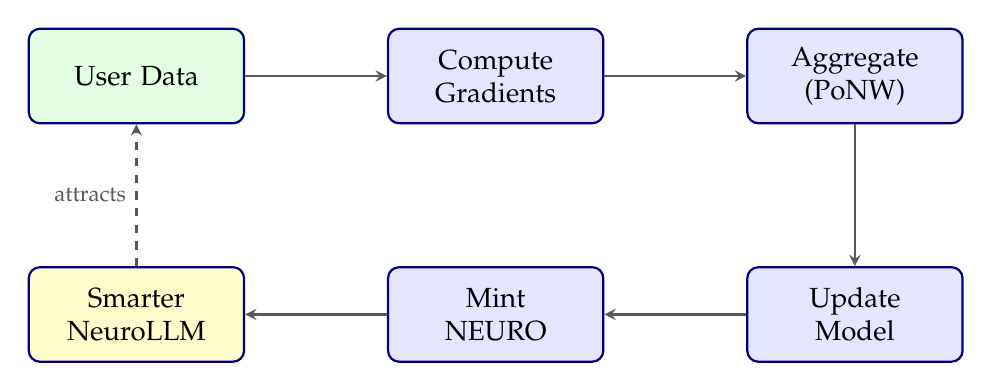
\begin{tikzpicture}[
    node distance=1.8cm,
    auto,
    block/.style={
        rectangle,
        draw=blue!50!black,
        thick,
        fill=blue!10,
        text width=2.5cm,
        align=center,
        rounded corners,
        minimum height=1.2cm
    },
    arrow/.style={
        ->,
        >=stealth,
        thick,
        color=gray!70!black
    }
]

% Nodes in a cycle
\node[block, fill=green!10] (data) {User Data};
\node[block, right=of data] (gradient) {Compute\\Gradients};
\node[block, right=of gradient] (aggregate) {Aggregate\\(PoNW)};
\node[block, below=of aggregate] (update) {Update\\Model};
\node[block, left=of update] (reward) {Mint\\NEURO};
\node[block, left=of reward, fill=yellow!20] (model) {Smarter\\NeuroLLM};

% Arrows
\draw[arrow] (data) -- (gradient);
\draw[arrow] (gradient) -- (aggregate);
\draw[arrow] (aggregate) -- (update);
\draw[arrow] (update) -- (reward);
\draw[arrow] (reward) -- (model);
\draw[arrow, dashed] (model) -- node[left, font=\footnotesize] {attracts} (data);

\end{tikzpicture}
\caption{PoNW Cycle: User data → Gradients → Aggregation → Model Update → NEURO Rewards → Smarter Model → More Users}
\label{fig:ponw-cycle}
\end{figure}

This creates a \textbf{virtuous cycle}:
\begin{enumerate}
    \item Users contribute data and compute
    \item PoNW validates contributions and mints NEURO
    \item Model improves with each training round
    \item Better model attracts more users
    \item More users = more data = faster improvement
\end{enumerate}

\subsection{PoNW Components}

PoNW validates three types of work:

    \begin{enumerate}
    \item \textbf{Proof of Inference:} Tokens processed during text generation. Each forward pass through NeuroLLM is counted.
    \item \textbf{Proof of Training:} Gradient contributions to model improvement. The gradient's impact on loss reduction is measured.
    \item \textbf{Proof of Data:} Training samples contributed. Data quality is assessed by the resulting gradient quality.
    \end{enumerate}

\subsection{The Training-Mining Equivalence}

In NeuroShard, \textbf{training IS mining}. Traditional cryptocurrency mining wastes energy on arbitrary computation. NeuroShard redirects that energy into building collective intelligence:

\begin{table}[H]
\centering
\caption{Mining Comparison}
\begin{tabular}{@{}lll@{}}
\toprule
\textbf{Aspect} & \textbf{Bitcoin (PoW)} & \textbf{NeuroShard (PoNW)} \\
\midrule
Work Type & SHA-256 hashing & Neural network training \\
Output & Block hash & Model improvement \\
Useful? & No (arbitrary) & Yes (builds AI) \\
Verification & Hash check & Loss reduction \\
Energy Use & Wasted & Productive \\
\bottomrule
\end{tabular}
\end{table}

Every NEURO token represents real intelligence added to NeuroLLM. The token's value is backed by the model's capability.

\subsection{Reward Function}

The total NEURO reward for a Proof of Neural Work is calculated as:

\begin{equation}
R_{\text{total}} = \left( R_{\text{uptime}} + R_{\text{inference}} + R_{\text{training}} + R_{\text{data}} \right) \cdot M_{\text{role}} \cdot M_{\text{stake}} \cdot M_{\text{training}}
\end{equation}

Where the base rewards are:
\begin{itemize}
    \item $R_{\text{uptime}} = 0.0001 \cdot \frac{T_{\text{seconds}}}{60}$ NEURO (uptime, minimal)
    \item $R_{\text{inference}} = 0.1 \cdot \frac{T_{\text{tokens}}}{10^6} \cdot S_{\text{role}}$ NEURO (role-weighted inference)
    \item $R_{\text{training}} = 0.0005 \cdot B_{\text{batches}}$ NEURO (training batches, dominant)
    \item $R_{\text{data}} = 0.00001 \cdot D_{\text{samples}}$ NEURO (data serving)
\end{itemize}

And the multipliers are:
\begin{itemize}
    \item $M_{\text{role}} = 1.0 + \text{LayerBonus} + \text{DriverBonus} + \text{ValidatorBonus}$
    \item $M_{\text{stake}} = 1.0 + 0.1 \cdot \log_2\left(1 + \frac{S_{\text{stake}}}{1000}\right)$ (diminishing returns, see Section~\ref{sec:diminishing-returns})
    \item $M_{\text{training}} = 1.1$ if actively training, else $1.0$
\end{itemize}

The role share $S_{\text{role}}$ for inference is:
\begin{itemize}
    \item Driver (has embedding): $S_{\text{role}} = 0.15$
    \item Worker (middle layers): $S_{\text{role}} = 0.70$
    \item Validator (has LM head): $S_{\text{role}} = 0.15$
\end{itemize}

\subsection{Proof Generation}

Nodes generate PoNW proofs every 60 seconds:

\begin{lstlisting}[caption=PoNW Proof Generation]
def get_ponw_proof(self) -> Dict:
    proof = {
        "node_id": self.node_id,
        "timestamp": time.time(),
        "tokens_processed": self.total_tokens_processed,
        "training_rounds": self.total_training_rounds,
        "layers_held": len(self.my_layer_ids),
        "reward_multiplier": self.calculate_reward_multiplier(),
    }
    
    # Sign the proof
    proof_string = f"{self.node_id}:{proof['timestamp']}:{proof['layers_held']}"
    proof["signature"] = sha256(proof_string).hexdigest()
    
    return proof
\end{lstlisting}

\subsection{Proof Validation}

Receiving nodes validate proofs by checking:

\begin{enumerate}
    \item \textbf{Signature:} Cryptographically valid
    \item \textbf{Timestamp:} Within 5-minute window (prevents replay)
    \item \textbf{Non-duplicate:} Not already processed
    \item \textbf{Plausibility:} Token counts are reasonable for the time period
\end{enumerate}

\subsection{Gradient Verification}

The core innovation of PoNW is \textbf{gradient verification}. When a node submits a gradient contribution, it can be verified through:

\subsubsection{Statistical Verification}
Valid gradients have predictable statistical properties:
\begin{itemize}
    \item \textbf{Distribution:} Real gradients follow a roughly Gaussian distribution
    \item \textbf{Magnitude:} Gradient norms fall within expected ranges based on batch size
    \item \textbf{Sparsity:} After Top-K compression, valid gradients have specific sparsity patterns
\end{itemize}

\subsubsection{Loss-Based Verification}
The ultimate test of a gradient's validity is whether it reduces loss:
\begin{equation}
\mathcal{L}(w - \eta \cdot g) < \mathcal{L}(w)
\end{equation}

Where $w$ is the current weights, $\eta$ is the learning rate, and $g$ is the submitted gradient. If this inequality holds on a validation set, the gradient is valid.

\subsubsection{Cross-Validation}
Multiple nodes computing gradients on similar data should produce similar gradients. Outliers are flagged:
\begin{equation}
\text{score}(g_i) = \frac{\|g_i - \bar{g}\|}{\sigma_g}
\end{equation}

Gradients with $\text{score} > 3$ (more than 3 standard deviations from mean) are rejected.

\subsection{Attack Prevention}

PoNW prevents common attacks through a multi-layered security model:

\begin{itemize}
    \item \textbf{Freeloading:} Cannot earn rewards without running the model and computing real gradients
    \item \textbf{Inflation:} Token counts are cross-validated against actual computation time
    \item \textbf{Sybil:} Staking requirement (1000 NEURO) makes fake nodes expensive
    \item \textbf{Gradient Poisoning:} Robust aggregation and statistical verification reject malicious gradients
    \item \textbf{Replay Attacks:} Timestamp windows and signature uniqueness prevent proof reuse
\end{itemize}

\subsection{Cryptographic Security Model}

Every PoNW proof is cryptographically secured using \textbf{ECDSA (secp256k1)}:

\begin{enumerate}
    \item \textbf{BIP39 Wallet:} Users generate a 12-word mnemonic seed phrase (similar to MetaMask). The node token is derived as $\text{token} = \text{BIP39\_seed}(\text{mnemonic})[:32]$. Private keys are never stored---only the user controls their wallet.
    \item \textbf{Key Derivation:} $\text{private\_key} = \text{SHA256}(\text{node\_token})$ (32 bytes)
    \item \textbf{Public Key:} $\text{public\_key} = \text{ECDSA.derive}(\text{private\_key})$ (33 bytes compressed)
    \item \textbf{Node Identity:} $\text{node\_id} = \text{SHA256}(\text{public\_key})[:32]$ (deterministic from public key)
    \item \textbf{Proof Signature:} $\text{sig} = \text{ECDSA.sign}(\text{private\_key}, \text{canonical\_payload})$
    \item \textbf{Trustless Verification:} Anyone can verify signatures using only the public key
    \item \textbf{Timestamp Freshness:} Proofs must be $<$ 5 minutes old
    \item \textbf{Replay Prevention:} Each signature stored in \texttt{proof\_history}, can never be reused
    \item \textbf{Rate Limiting:} Max 120 proofs/hour, max 1M tokens/minute per node
\end{enumerate}

\textbf{Why ECDSA over HMAC?} HMAC requires sharing the secret token to verify signatures. ECDSA allows \textbf{trustless verification} - any node can verify a proof's authenticity using only the signer's public key, without needing their secret token. This is essential for decentralized consensus.

The canonical payload format ensures deterministic verification:
\begin{verbatim}
payload = f"{node_id}:{proof_type}:{timestamp}:{nonce}:
            {uptime}:{tokens}:{batches}:{samples}:
            {layers}:{has_embed}:{has_head}"
\end{verbatim}

\textbf{Transparency Guarantee:} There is NO admin backdoor. The ONLY way to get NEURO is to run a node, do real work, create a signed proof, and pass ALL verification checks. Even the project creators must run nodes and earn like everyone else.

\section{Hybrid Validator System}
\label{sec:hybrid-validators}

NeuroShard introduces a novel \textbf{Hybrid Validator} model that combines the best aspects of Proof of Work (computational contribution) and Proof of Stake (economic commitment) into a unified validation system. This hybrid approach solves critical problems that neither mechanism can address alone.

\subsection{The Problem with Pure Approaches}

\subsubsection{Pure Proof of Work Limitations}
In a pure PoW system for neural networks:
\begin{itemize}
    \item \textbf{No Economic Stake:} Malicious nodes can submit poisoned gradients with no financial risk
    \item \textbf{Sybil Vulnerability:} Attackers can spin up many nodes cheaply
    \item \textbf{No Accountability:} Bad actors can simply restart with new identities
\end{itemize}

\subsubsection{Pure Proof of Stake Limitations}
In a pure PoS system:
\begin{itemize}
    \item \textbf{Rich-Get-Richer:} Large stakeholders dominate rewards exponentially
    \item \textbf{No Work Required:} Validators can earn without contributing compute
    \item \textbf{Centralization:} Wealth concentration leads to validator monopolies
\end{itemize}

\subsection{The Hybrid Solution}

NeuroShard's Hybrid Validator combines \textbf{Model Validation} (layer-based work) with \textbf{Consensus Validation} (stake-based verification):

\begin{figure}[H]
\centering
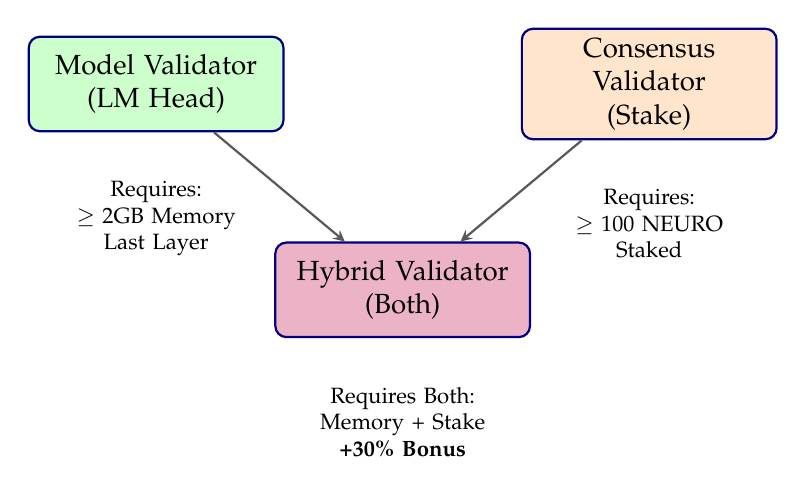
\begin{tikzpicture}[
    node distance=1.5cm,
    auto,
    block/.style={
        rectangle,
        draw=blue!50!black,
        thick,
        fill=blue!10,
        text width=3cm,
        align=center,
        rounded corners,
        minimum height=1.2cm
    },
    arrow/.style={
        ->,
        >=stealth,
        thick,
        color=gray!70!black
    }
]

% Model Validator side
\node[block, fill=green!20] (model) {Model Validator\\(LM Head)};
\node[below=0.5cm of model, text width=3cm, align=center, font=\footnotesize] (model_req) {Requires:\\$\geq$ 2GB Memory\\Last Layer};

% Consensus Validator side
\node[block, fill=orange!20, right=3cm of model] (consensus) {Consensus Validator\\(Stake)};
\node[below=0.5cm of consensus, text width=3cm, align=center, font=\footnotesize] (cons_req) {Requires:\\$\geq$ 100 NEURO\\Staked};

% Hybrid Validator
\node[block, fill=purple!30, below=2cm of $(model)!0.5!(consensus)$] (hybrid) {Hybrid Validator\\(Both)};
\node[below=0.5cm of hybrid, text width=4cm, align=center, font=\footnotesize] (hybrid_req) {Requires Both:\\Memory + Stake\\\textbf{+30\% Bonus}};

% Arrows
\draw[arrow] (model) -- (hybrid);
\draw[arrow] (consensus) -- (hybrid);

\end{tikzpicture}
\caption{Hybrid Validator combines Model Validation (compute) with Consensus Validation (stake)}
\label{fig:hybrid-validator}
\end{figure}

\subsubsection{Validator Requirements}
To become a Hybrid Validator, a node must meet \textbf{both} requirements:

\begin{table}[H]
\centering
\caption{Hybrid Validator Requirements}
\begin{tabular}{@{}lll@{}}
\toprule
\textbf{Requirement} & \textbf{Type} & \textbf{Purpose} \\
\midrule
$\geq$ 2GB Memory & Compute & Hold LM Head layer \\
$\geq$ 100 NEURO Staked & Economic & Skin in the game \\
Last Layer Assignment & Network & Model validation role \\
\bottomrule
\end{tabular}
\end{table}

\subsubsection{Dual Responsibilities}
Hybrid Validators perform two critical functions:

\begin{enumerate}
    \item \textbf{Model Validation:} Compute loss on the final layer, initiate backward pass, verify gradient quality
    \item \textbf{Consensus Validation:} Verify PoNW proofs from other nodes, cast stake-weighted votes, participate in consensus
\end{enumerate}

\subsection{Stake-Weighted Proof Validation}

When a node submits a PoNW proof, Hybrid Validators verify it through a stake-weighted voting system:

\begin{algorithm}[H]
\caption{Stake-Weighted Proof Validation}
\begin{algorithmic}[1]
\Procedure{ValidateProof}{$proof$}
    \State $validators \gets \text{SelectValidators}(proof, n=3)$ \Comment{Stake-weighted random}
    \For{$v \in validators$}
        \State $vote_v \gets v.\text{ValidateLocally}(proof)$ \Comment{Check plausibility}
        \State $\text{GossipVote}(proof, vote_v, v.stake)$
    \EndFor
    \State $valid\_stake \gets \sum_{v: vote_v = \text{true}} v.stake$
    \State $total\_stake \gets \sum_v v.stake$
    \If{$\frac{valid\_stake}{total\_stake} \geq 0.66$} \Comment{66\% threshold}
        \State $\text{ProcessProof}(proof)$ \Comment{Credit rewards}
    \Else
        \State $\text{RejectProof}(proof)$
    \EndIf
\EndProcedure
\end{algorithmic}
\end{algorithm}

\subsubsection{Validator Selection}
Validators are selected using a \textbf{stake-weighted random} algorithm that balances fairness with security:

\begin{equation}
\text{Score}_i = \text{Stake}_i \times (1 - r) + \text{Random}_i \times r \times \text{MaxStake}
\end{equation}

Where $r = 0.3$ (30\% randomness factor). This ensures:
\begin{itemize}
    \item Higher stake = higher chance of selection (security)
    \item Randomness prevents stake monopolies (fairness)
    \item Small stakers still get validation opportunities (decentralization)
\end{itemize}

\subsection{Diminishing Stake Returns}
\label{sec:diminishing-returns}

To prevent the ``rich-get-richer'' problem inherent in pure PoS systems, NeuroShard implements \textbf{logarithmic diminishing returns} on stake multipliers:

\begin{equation}
M_{\text{stake}} = 1.0 + 0.1 \times \log_2\left(1 + \frac{S_{\text{stake}}}{1000}\right)
\end{equation}

\begin{table}[H]
\centering
\caption{Diminishing Returns vs Linear Staking}
\begin{tabular}{@{}rrrr@{}}
\toprule
\textbf{Stake (NEURO)} & \textbf{Linear (Old)} & \textbf{Diminishing (New)} & \textbf{Reduction} \\
\midrule
1,000 & 1.10x & 1.10x & 0\% \\
2,000 & 1.20x & 1.16x & 3\% \\
5,000 & 1.50x & 1.26x & 16\% \\
10,000 & 2.00x & 1.35x & 33\% \\
50,000 & 6.00x & 1.56x & 74\% \\
100,000 & 11.00x & 1.66x & 85\% \\
\bottomrule
\end{tabular}
\end{table}

\textbf{Key Insight:} Under the old linear system, a whale with 100,000 NEURO would earn 11x rewards. Under diminishing returns, they earn only 1.66x. This dramatically reduces wealth concentration while still rewarding commitment.

\subsection{Validator Economics}

\subsubsection{Validator Rewards}
Hybrid Validators earn from multiple sources:

\begin{table}[H]
\centering
\caption{Validator Reward Sources}
\begin{tabular}{@{}llr@{}}
\toprule
\textbf{Source} & \textbf{Description} & \textbf{Rate} \\
\midrule
Model Validation & LM Head computation & +30\% bonus \\
Proof Validation & Per proof validated & 0.001 NEURO \\
Stake Multiplier & Diminishing returns & up to 1.66x \\
Training Bonus & If actively training & +10\% \\
\bottomrule
\end{tabular}
\end{table}

\subsubsection{Validator Slashing}
Validators who vote against consensus are \textbf{slashed at 2x the normal rate}:

\begin{equation}
\text{Slash}_{\text{validator}} = \text{Slash}_{\text{base}} \times 2.0 = 20 \text{ NEURO}
\end{equation}

The slashed amount is burned, creating deflationary pressure. This ensures:
\begin{itemize}
    \item Validators have strong incentive to vote honestly
    \item Bad validators lose their stake (can no longer validate)
    \item The cost of attacking consensus scales with stake
\end{itemize}

\subsection{Why Hybrid Validators Work}

The Hybrid Validator model solves the fundamental tension between decentralization and security:

\begin{enumerate}
    \item \textbf{Work Dominates:} You cannot earn significant rewards without actual computation (training, inference). Stake only provides a multiplier, not base rewards.
    
    \item \textbf{Stake Provides Accountability:} Validators have economic skin in the game. Cheating costs real money.
    
    \item \textbf{Diminishing Returns Prevent Monopolies:} Whales cannot dominate through pure capital. A node with 100x more stake only gets 1.5x more rewards.
    
    \item \textbf{Low Barrier to Entry:} Only 100 NEURO required to become a validator. This is earnable in $\sim$1 week of active participation.
    
    \item \textbf{Random Selection Ensures Fairness:} 30\% randomness means small validators still get opportunities to validate and earn fees.
\end{enumerate}

\begin{figure}[H]
\centering
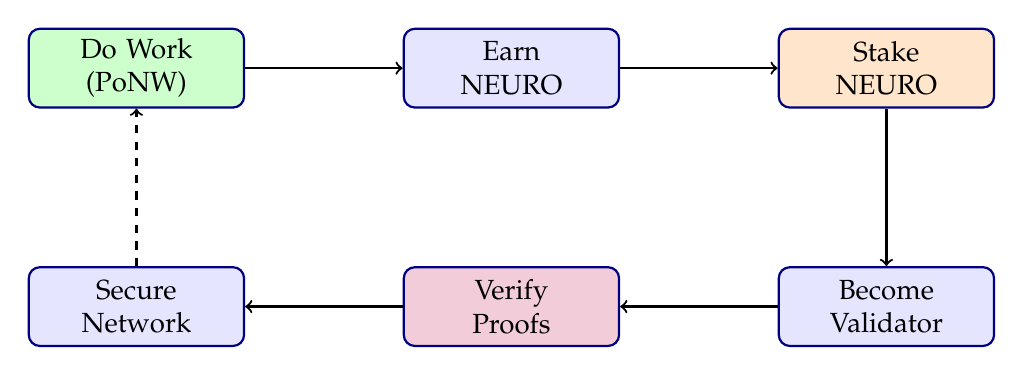
\begin{tikzpicture}[
    node distance=2cm,
    auto,
    block/.style={
        rectangle,
        draw=blue!50!black,
        thick,
        fill=blue!10,
        text width=2.5cm,
        align=center,
        rounded corners,
        minimum height=1cm
    }
]

% The virtuous cycle
\node[block, fill=green!20] (work) {Do Work\\(PoNW)};
\node[block, right=of work] (earn) {Earn\\NEURO};
\node[block, right=of earn, fill=orange!20] (stake) {Stake\\NEURO};
\node[block, below=of stake] (validate) {Become\\Validator};
\node[block, left=of validate, fill=purple!20] (verify) {Verify\\Proofs};
\node[block, left=of verify] (secure) {Secure\\Network};

\draw[->, thick] (work) -- (earn);
\draw[->, thick] (earn) -- (stake);
\draw[->, thick] (stake) -- (validate);
\draw[->, thick] (validate) -- (verify);
\draw[->, thick] (verify) -- (secure);
\draw[->, thick, dashed] (secure) -- (work);

\end{tikzpicture}
\caption{The Hybrid Validator Virtuous Cycle: Work → Earn → Stake → Validate → Secure → More Work}
\label{fig:validator-cycle}
\end{figure}

\textbf{The Result:} A system where validators are both computationally invested (they run the model) and economically invested (they stake tokens). This dual commitment creates the strongest possible incentive alignment for honest behavior.

\section{Robustness and Anti-Poisoning}

\subsection{The Model Poisoning Threat}
In a decentralized training environment, malicious actors may attempt to "poison" the model by submitting gradients that degrade performance or inject hidden backdoors (triggers). NeuroShard employs a multi-layered defense strategy.

\subsection{Robust Aggregation}
To secure the global model against adversarial attacks ("poisoning"), the Training Coordinator employs \textbf{Robust Aggregation} algorithms rather than simple averaging.

\begin{itemize}
    \item \textbf{Trimmed Mean:} For each parameter coordinate, the highest and lowest $k\%$ of values are discarded before averaging. This neutralizes outliers.
    \item \textbf{Coordinate-wise Median:} The median value of gradients is used, which theoretically tolerates up to 50\% malicious participants.
    \item \textbf{Krum/Bulyan:} Advanced selection algorithms that identify the gradient vector closest to the spatial center of the distribution.
\end{itemize}

\subsection{The Fraud Proof System}
To address the "Lazy Verifier" problem and ensure economic security, NeuroShard implements a challenge-response system:
\begin{itemize}
    \item \textbf{Evidence Submission:} If a node detects a statistically anomalous gradient (e.g., $>5\sigma$ deviation), it generates a cryptographic \textbf{Fraud Proof}.
    \item \textbf{Verification:} The proof, containing the signed malicious gradient and statistical context, is broadcast to the network.
    \item \textbf{Slashing:} Upon verification, the malicious node's staked NEURO is slashed.
\end{itemize}

\section{Governance and The NeuroDAO}

NeuroLLM is not a static artifact; it is a living system that must evolve. Governance is handled by the \textbf{NeuroDAO}.

\subsection{What NeuroDAO Does NOT Control}
Unlike traditional systems, NeuroDAO does \textbf{not} vote on:
\begin{itemize}
    \item \textbf{Model Size:} This is determined automatically by network capacity
    \item \textbf{Phase Transitions:} There are no phases - the model grows organically
    \item \textbf{Who Can Participate:} Anyone with compute can join
\end{itemize}

\subsection{What NeuroDAO Controls}
NEURO token holders vote on:
\begin{itemize}
    \item \textbf{Reward Rates:} Adjusting the $R_{compute}$ and $R_{data}$ multipliers to balance supply and demand.
    \item \textbf{Slashing Conditions:} Defining what constitutes malicious behavior and the penalties.
    \item \textbf{Protocol Parameters:} Minimum stake, gradient compression ratio, training round duration.
\end{itemize}

\subsection{Model Architecture Governance}
The community decides on the ``brain structure'' of NeuroLLM:
\begin{itemize}
    \item \textbf{Tokenizer Updates:} Voting to add new tokens to the vocabulary (e.g., for new languages or coding frameworks).
    \item \textbf{Architecture Changes:} Proposals to switch from RoPE to ALiBi, or introduce Mixture-of-Experts layers, are submitted as Neuro Improvement Proposals (NIPs).
    \item \textbf{Layer Architecture:} Changes to attention mechanism, FFN structure, or normalization.
\end{itemize}

\section{NEURO Token Economics}

\subsection{Token Utility}

The NEURO token serves four functions:

\begin{enumerate}
    \item \textbf{Reward Currency:} Earned by contributing compute and data
    \item \textbf{Payment Currency:} Spent to access NeuroLLM inference
    \item \textbf{Staking Security:} Staked to earn reward multipliers (with diminishing returns)
    \item \textbf{Validator Eligibility:} Minimum 100 NEURO stake required to become a Hybrid Validator
\end{enumerate}

\subsection{Genesis Block and Transparency}

NeuroShard's ledger is initialized with a \textbf{Genesis Block} that guarantees zero pre-mine:

\begin{itemize}
    \item \textbf{Zero Pre-Mine:} The ledger starts with \texttt{total\_minted = 0.0}
    \item \textbf{No Founder Allocation:} There are no pre-allocated tokens for founders or investors
    \item \textbf{No ICO:} All NEURO must be earned through verified Proof of Neural Work
    \item \textbf{Audit Trail:} Every token minted is traceable to a specific PoNW proof
\end{itemize}

The Genesis Block is recorded in the \texttt{proof\_history} table with signature \texttt{GENESIS\_BLOCK} and reward amount \texttt{0.0}. Anyone can verify this by querying:
\begin{verbatim}
SELECT * FROM global_stats WHERE id = 1;
-- Returns: total_minted=0.0, total_burned=0.0 (at genesis)
\end{verbatim}

\subsection{Deflationary Mechanics}
To ensure long-term value accrual, NeuroShard implements a \textbf{Burn Mechanism}:
\begin{itemize}
    \item \textbf{Fee Burn:} 5\% of all spending (inference, transfers) is permanently burned
    \item \textbf{Fraud Slashing:} 50\% of slashed stakes from malicious nodes are burned (50\% to whistleblower)
    \item \textbf{Validator Slashing:} 100\% of validator slashes are burned (validators slashed at 2x rate for voting against consensus)
    \item \textbf{Burn Address:} \texttt{BURN\_0x0000...} - tokens sent here are irrecoverable
\end{itemize}
As network usage grows, the supply of NEURO decreases, rewarding long-term holders and contributors.

\subsection{Earning NEURO}

Users earn NEURO through a hierarchical reward structure that prioritizes \textbf{Training} as the core value:

\begin{table}[H]
\centering
\caption{NEURO Earning Mechanisms (Reward Hierarchy)}
\begin{tabular}{@{}llrl@{}}
\toprule
\textbf{Activity} & \textbf{Description} & \textbf{Rate} & \textbf{Daily (Active)} \\
\midrule
\textbf{Training} & Contributing gradients & 0.0005 NEURO/batch & $\sim$43 NEURO \\
Inference & Processing tokens & Market-based (pure supply/demand) & Variable \\
Data & Serving training shards & 0.00001 NEURO/sample & Variable \\
Uptime & Running a node (idle) & 0.0001 NEURO/min & $\sim$0.14 NEURO \\
\bottomrule
\end{tabular}
\end{table}

\textbf{Note on Dynamic Pricing:} Inference rewards use a \textbf{pure market} where price is determined by supply and demand. When the model is worthless (bootstrap), demand is zero and price approaches zero. As the model improves and attracts users, demand rises naturally and price increases. The market self-regulates: high prices attract more nodes to inference, while low prices push nodes back to training. Quality emerges from the demand signal itself.

\subsubsection{Privacy-Preserving Distributed Inference Marketplace}

NeuroShard implements a \textbf{request-response marketplace} that orchestrates distributed inference while preserving user privacy.

\textbf{Architecture:}

Inference in NeuroShard is inherently distributed across the pipeline:
\begin{enumerate}
    \item \textbf{User} submits request to marketplace (metadata only - NO prompt!)
    \item \textbf{Driver node} (Layer 0) receives encrypted prompt directly from user
    \item \textbf{Worker nodes} (Layers 1-N) process activations (never see prompt)
    \item \textbf{Validator node} (LM Head) generates output, returns to user
\end{enumerate}

\textbf{Privacy Guarantee:} The prompt is NEVER stored in the marketplace. Users send encrypted prompts directly to their chosen driver node via a private channel. Worker nodes only process activations (meaningless vector representations), ensuring they cannot reconstruct the original prompt. This preserves privacy while enabling distributed computation.

\textbf{Pure Market Pricing (No Artificial Caps):}
\begin{equation}
P_{\text{market}} = P_{\text{base}} \times (1 + u)^2
\end{equation}

Where:
\begin{itemize}
    \item $P_{\text{base}} = 0.0001$ NEURO (starting price)
    \item $u = \text{demand rate} / \text{supply rate}$ (utilization)
    \item NO minimum or maximum caps - market finds true value
\end{itemize}

\textbf{Request-Response Matching:}

To prevent timing attacks, prices are \textbf{locked at submission time}:
\begin{enumerate}
    \item User submits request → Price locked at current market rate
    \item Driver claims request → Starts distributed pipeline
    \item All nodes submit proofs → Each rewarded by role
    \item Request marked complete → All participants paid at locked price
\end{enumerate}

This ensures users always pay the price they saw at submission, even if market price spikes during processing.

\textbf{Distributed Reward Distribution:}

Multiple nodes participate in each inference request. The locked price determines the total reward pool, distributed by role:
\begin{itemize}
    \item \textbf{Driver (Layer 0):} 15\% of pool (processes embedding, sees prompt)
    \item \textbf{Workers (Layers 1-N):} 70\% of pool (divided among participants)
    \item \textbf{Validator (LM Head):} 15\% of pool (generates output)
\end{itemize}

Each node submits its own signed PoNW proof linking to the same \texttt{request\_id}. The ledger validates all proofs and distributes rewards accordingly.

\textbf{Market Dynamics:}
\begin{itemize}
    \item \textbf{Worthless model:} No demand → Price $\approx$ 0 (nodes focus on training)
    \item \textbf{Improving model:} Rising demand → Price increases naturally
    \item \textbf{Viral demand:} Price spikes → Attracts more inference capacity
    \item \textbf{Equilibrium:} Market self-regulates where training profit $\gg$ inference profit
\end{itemize}

\textbf{Key Properties:}
\begin{enumerate}
    \item \textbf{Privacy:} Workers never see prompts, only activations
    \item \textbf{Decentralization:} Uses existing pipeline parallelism architecture
    \item \textbf{Fair pricing:} Price locked at submission (no timing attacks)
    \item \textbf{Quality signal:} Demand IS quality (no manual adjustments needed)
    \item \textbf{Self-regulation:} Market finds equilibrium automatically
\end{enumerate}

This marketplace enables NeuroShard to provide inference services while maintaining its core principles of privacy, decentralization, and fair compensation.

\subsubsection{Multipliers and Bonuses}
\begin{table}[H]
\centering
\caption{Reward Multipliers}
\begin{tabular}{@{}llr@{}}
\toprule
\textbf{Multiplier} & \textbf{Condition} & \textbf{Bonus} \\
\midrule
Staking Bonus & Diminishing: $\log_2(1 + S/1000)$ & up to +66\% \\
Training Bonus & Actively training & +10\% rewards \\
Driver Bonus & Holding embedding layer & +20\% rewards \\
Validator Bonus & Holding LM head + 100 NEURO stake & +30\% rewards \\
Layer Bonus & Per layer held & +5\% (max 100\%) \\
Validation Fee & Per proof validated & 0.001 NEURO \\
\bottomrule
\end{tabular}
\end{table}

\textbf{Note:} The Validator Bonus increased from 20\% to 30\% to compensate for the additional stake requirement and proof validation responsibilities.

\subsection{Spending NEURO}

Users spend NEURO for:

\begin{itemize}
    \item \textbf{Inference:} 1 NEURO per 1M tokens generated
    \item \textbf{Priority:} Higher payment for faster processing
    \item \textbf{Transfers:} Send NEURO to other users
\end{itemize}

\subsection{Economic Equilibrium}

The system creates a sustainable economy:

\begin{itemize}
    \item \textbf{Active Contributors:} Earn more than they spend
    \item \textbf{Passive Users:} Must purchase NEURO to use the service
    \item \textbf{Network Effect:} More users → more training → better model → more users
\end{itemize}

\section{Security Considerations}

\subsection{Threat Model}

NeuroShard assumes:
\begin{itemize}
    \item Up to 49\% of nodes may be malicious
    \item Attackers are economically rational
    \item Cryptographic primitives are secure
\end{itemize}

\subsection{Data Privacy}

Training data is protected through:
\begin{itemize}
    \item \textbf{Local Processing:} Raw data never leaves the node
    \item \textbf{Differential Privacy:} Token-level noise injection
    \item \textbf{Gradient Compression:} Only sparse gradients are shared
\end{itemize}

\subsection{Model Integrity}

NeuroLLM integrity is maintained through:
\begin{itemize}
    \item \textbf{Gradient Validation:} Anomalous gradients are rejected
    \item \textbf{Checkpoint Hashing:} Model state is cryptographically verified
    \item \textbf{Consensus:} Updates require majority agreement
\end{itemize}

\subsection{Sybil Resistance}

Sybil attacks are prevented through multiple layers:
\begin{itemize}
    \item \textbf{Validator Stake:} 100 NEURO minimum to become a Hybrid Validator (verify proofs)
    \item \textbf{PoNW Requirement:} Must actually run the model to earn base rewards (stake only provides multiplier)
    \item \textbf{Diminishing Returns:} Creating 10 nodes with 100 NEURO each yields less than 1 node with 1000 NEURO
    \item \textbf{Slashing Risk:} Malicious validators lose their stake (2x penalty)
    \item \textbf{ECDSA Identity:} Node IDs derived from public keys prevent identity spoofing
\end{itemize}

\section{Checkpoint System and State Sharding}

\subsection{Sharded Checkpoints}

Unlike centralized systems where the full model state exists on a single disk, NeuroShard utilizes a \textbf{Sharded Checkpoint} system. The global model state is partitioned, with each node responsible for persisting only the weights of its assigned layers.

\begin{itemize}
    \item \textbf{Distributed Storage:} No single node needs to store the entire multi-terabyte model file.
    \item \textbf{Redundancy:} Each shard is replicated across multiple nodes (based on layer assignment redundancy).
    \item \textbf{Merkle Integrity:} A root Merkle hash ensures the consistency of the global state across all shards without requiring full assembly.
\end{itemize}

\subsection{Checkpoint Structure}

Each node maintains a local shard:

\begin{lstlisting}[caption=Sharded Checkpoint Structure]
shard = {
    "shard_id": "hash_of_node_id",
    "version": 1234,
    "layer_ids": [0, 1, 2, ...],     # Specific layers held by this node
    "state_dict": {...},             # Weights for ONLY these layers
    "optimizer_state": {...},        # Optimizer state for these layers
    "model_hash": "sha256...",       # Hash of this shard
    "timestamp": 1712345678
}
\end{lstlisting}

This approach allows the network to persist models that are significantly larger than the storage capacity of any individual participant.

\subsection{Checkpoint Synchronization}

New nodes joining the network synchronize via:

\begin{enumerate}
    \item \textbf{Discovery:} Query DHT for nodes with latest checkpoint version
    \item \textbf{Download:} Fetch checkpoint from multiple peers (parallel chunks)
    \item \textbf{Verification:} Verify hash matches consensus
    \item \textbf{Load:} Initialize NeuroLLM from checkpoint
\end{enumerate}

\subsection{Model Evolution Over Time}

NeuroLLM evolves through two mechanisms:

\subsubsection{Continuous Training}
Every 60 seconds, a training round completes:
\begin{itemize}
    \item Gradients from all contributing nodes are aggregated
    \item Model weights are updated
    \item New checkpoint is created
    \item NEURO rewards are distributed
\end{itemize}

\subsubsection{Organic Growth}
As more nodes join, the model automatically grows:
\begin{enumerate}
    \item New node joins with available memory
    \item Network assigns new layers to the node
    \item Model capacity increases
    \item Training continues on larger architecture
\end{enumerate}

\textbf{No votes required.} The model grows as naturally as the network grows. A node with 16GB RAM joining the network immediately increases the model's capacity by $\sim$156 layers.

\subsubsection{Architecture Upgrades}
The community can vote on architectural improvements:
\begin{itemize}
    \item Adding new attention mechanisms
    \item Expanding vocabulary (new tokens)
    \item Introducing specialized experts (MoE)
\end{itemize}

\subsection{The Intelligence Ledger}

Every improvement to NeuroLLM is recorded in an \textbf{Intelligence Ledger}:

\begin{table}[H]
\centering
\caption{Intelligence Ledger Entry}
\begin{tabular}{@{}ll@{}}
\toprule
\textbf{Field} & \textbf{Description} \\
\midrule
Round ID & Unique training round identifier \\
Timestamp & When the round completed \\
Contributors & List of node IDs that contributed \\
Batch Size & Total samples processed \\
Loss Before & Model loss before update \\
Loss After & Model loss after update \\
NEURO Minted & Total tokens distributed \\
Checkpoint Hash & Hash of resulting model state \\
\bottomrule
\end{tabular}
\end{table}

This creates an immutable record of how NeuroLLM was built - every contribution, every improvement, every NEURO token can be traced back to specific training rounds.

\section{Implementation}

\subsection{Technology Stack}

\begin{itemize}
    \item \textbf{PyTorch:} Neural network framework
    \item \textbf{FastAPI:} HTTP API server
    \item \textbf{gRPC:} Inter-node communication
    \item \textbf{Tkinter:} Desktop GUI
    \item \textbf{Kademlia:} DHT implementation
    \item \textbf{PyInstaller:} Cross-platform packaging
\end{itemize}

\subsection{API Endpoints}

\begin{table}[H]
\centering
\caption{NeuroNode API Endpoints}
\begin{tabular}{@{}lll@{}}
\toprule
\textbf{Endpoint} & \textbf{Method} & \textbf{Description} \\
\midrule
/generate\_text & POST & Generate text from prompt \\
/contribute\_data & POST & Add training data \\
/train\_step & POST & Trigger training step \\
/training\_status & GET & Get training metrics \\
/api/stats & GET & Node statistics \\
/api/ponw & GET & Get PoNW proof \\
/api/model\_info & GET & Model information \\
\bottomrule
\end{tabular}
\end{table}

\subsection{Desktop Application}

The NeuroShard GUI provides:
\begin{itemize}
    \item One-click node startup
    \item Real-time training metrics
    \item NEURO balance display
    \item Training enable/disable toggle
    \item Automatic updates
\end{itemize}

\section{Vision and Roadmap}

NeuroShard's evolution is driven by network growth, not predetermined schedules. The following milestones represent capabilities that emerge naturally as participation increases.

\subsection{Foundation}
The core infrastructure for decentralized AI:
\begin{itemize}
    \item Dynamic layer pool for organic model scaling
    \item Gradient gossip protocol for decentralized training
    \item Proof of Neural Work consensus
    \item NEURO token economics
    \item Cross-platform node software (desktop, server)
\end{itemize}

\subsection{Robust Training}
Byzantine-tolerant training at scale:
\begin{itemize}
    \item Trimmed mean and median gradient aggregation
    \item Fraud proof mechanism with slashing
    \item Anomaly detection for gradient poisoning
    \item 50x+ gradient compression
    \item \textbf{Network Target:} 100+ active nodes
\end{itemize}

\subsection{Scale}
Optimizing for global-scale throughput:
\begin{itemize}
    \item \textbf{Mobile Optimization:} INT4 quantization and structural pruning for efficient edge device participation.
    \item \textbf{Hierarchical Aggregation:} Multi-tier parameter aggregation to minimize P2P latency in networks >10,000 nodes.
    \item \textbf{Developer SDK:} Comprehensive Python and JavaScript bindings for direct integration into third-party applications.
    \item \textbf{Network Target:} 1,000+ nodes, 1B+ parameters
\end{itemize}

\subsection{Maturity}
Global-scale collective intelligence:
\begin{itemize}
    \item Multi-modal capabilities (vision, audio, code)
    \item Specialized domain fine-tuning
    \item NeuroDAO governance for protocol decisions
    \item Enterprise and institutional integrations
    \item \textbf{Network Target:} 10,000+ nodes, 100B+ parameters
\end{itemize}

\textbf{Key Principle:} These are not ``phases'' requiring coordinated upgrades. They are capabilities that emerge as the network grows. A single node joining the network immediately increases model capacity.

\section{Distributed Architecture and Parallelism}

\subsection{The Dynamic Approach}

In NeuroShard, distributed inference is not a ``future feature'' - it is the \textbf{default architecture}. Each node holds only the layers it can support, and inference requests flow through the network:

\begin{itemize}
    \item Node A (2GB): Holds layers 0-18, including embedding
    \item Node B (4GB): Holds layers 19-56
    \item Node C (8GB): Holds layers 57-134
    \item Node D (4GB): Holds layers 135-172, including LM head
\end{itemize}

An inference request flows: Input $\rightarrow$ Node A $\rightarrow$ Node B $\rightarrow$ Node C $\rightarrow$ Node D $\rightarrow$ Output. Note that while the logical flow is linear, the physical routing is handled by the Swarm Network Layer (Section 16), where each step is dynamically routed to a redundant pool of peers to ensure fault tolerance.

\subsection{Advanced Parallelism}

NeuroShard implements advanced parallelism strategies to support massive models on consumer hardware.

\subsubsection{Tensor Parallelism}

To handle layers that are too large for a single device's memory (e.g., a 8192-dimension projection matrix), NeuroShard implements \textbf{Tensor Parallelism}. Large weight matrices are split across multiple nodes:

\begin{itemize}
    \item \textbf{Column Parallelism:} Dividing linear layers by output features.
    \item \textbf{Row Parallelism:} Dividing linear layers by input features.
\end{itemize}

This allows a single logical layer to span multiple physical devices, enabling the training of models with hidden dimensions far exceeding individual VRAM limits.

\subsubsection{Pipeline Parallelism}

As the default mode of operation, Pipeline Parallelism distributes the model vertically. Input activations flow through the network of nodes, each processing a subset of layers, similar to a packet moving through a network router chain. This naturally balances compute load across the heterogeneous cluster.

\subsection{Hybrid Parallelism}

For very large models, NeuroShard combines both approaches:
\begin{enumerate}
    \item \textbf{Inter-layer (Pipeline):} Different nodes hold different layers
    \item \textbf{Intra-layer (Tensor):} Large layers split across multiple nodes
\end{enumerate}

This enables models of \textbf{any size} to run across the network, each node contributing what it can.

\subsection{Training at Scale}

Distributed training uses:
\begin{itemize}
    \item \textbf{Gradient Accumulation:} Nodes accumulate gradients locally before sharing
    \item \textbf{Ring All-Reduce:} Efficient gradient synchronization across nodes
    \item \textbf{Asynchronous SGD:} Nodes can train at different speeds
    \item \textbf{Layer-Local Gradients:} Each node only computes gradients for its assigned layers
\end{itemize}

\subsection{The Key Insight}

Traditional distributed training requires homogeneous hardware and careful coordination. NeuroShard's dynamic layer pool allows \textbf{heterogeneous participation}:

\begin{itemize}
    \item A Raspberry Pi with 1GB RAM contributes 9 layers
    \item A gaming PC with 32GB RAM contributes 312 layers
    \item A cloud server with 256GB RAM contributes 2,500 layers
\end{itemize}

All participate in the same model, all earn NEURO proportional to contribution.

\section{Swarm Architecture: High-Latency Resilience}

\subsection{Design Philosophy: Throughput over Latency}

The core insight driving NeuroShard's network design is: \textbf{``Compute is cheap; Bandwidth is expensive.''} Residential internet connections (100Mbps-1Gbps) and node churn create fundamental challenges for distributed training. Rather than fighting these constraints, NeuroShard embraces them through an asynchronous, swarm-based architecture.

\textbf{Goal:} 95\% GPU utilization, even if wall-clock convergence is 10\% slower per epoch. We win by being \textit{unstoppable}, not by being the fastest.

\subsection{Swarm Network Layer (Fault-Tolerant Routing)}

Traditional pipeline parallelism fails catastrophically when any node in the chain becomes unresponsive. NeuroShard replaces the brittle linear pipeline with a \textbf{multipath routing system}.

\subsubsection{Key Directive}
``If Node A hangs, the packet must automatically flow to Node B without crashing the run.''

\subsubsection{Multipath Routing}

For each layer range, the DHT maintains a list of $K$ potential peers (typically $K=3$), sorted by a weighted score:

\begin{equation}
\text{Score}_i = w_{\text{latency}} \cdot \frac{\text{Latency}_i}{500\text{ms}} + w_{\text{queue}} \cdot \frac{\text{QueueDepth}_i}{100}
\end{equation}

Where $w_{\text{latency}} = 0.4$ and $w_{\text{queue}} = 0.6$. Lower scores indicate better candidates.

\subsubsection{Probabilistic Send with Failover}

When sending activations:
\begin{enumerate}
    \item Send to primary peer (lowest score)
    \item If no ACK within 200ms, immediately re-route to secondary peer
    \item Continue until success or all $K$ candidates exhausted
\end{enumerate}

This provides automatic failover without coordinator intervention.

\subsubsection{Capacity Bitmask Heartbeats}

Every 5 seconds, nodes broadcast a lightweight \textbf{Capacity Bitmask} ($\sim$20 bytes):
\begin{itemize}
    \item Available memory (MB)
    \item Current queue depth
    \item Layer range held
    \item GPU utilization (\%)
    \item Status flags (training/inference/accepting work)
\end{itemize}

This allows peers to know who is ready to receive work, enabling intelligent routing decisions.

\begin{figure}[H]
\centering
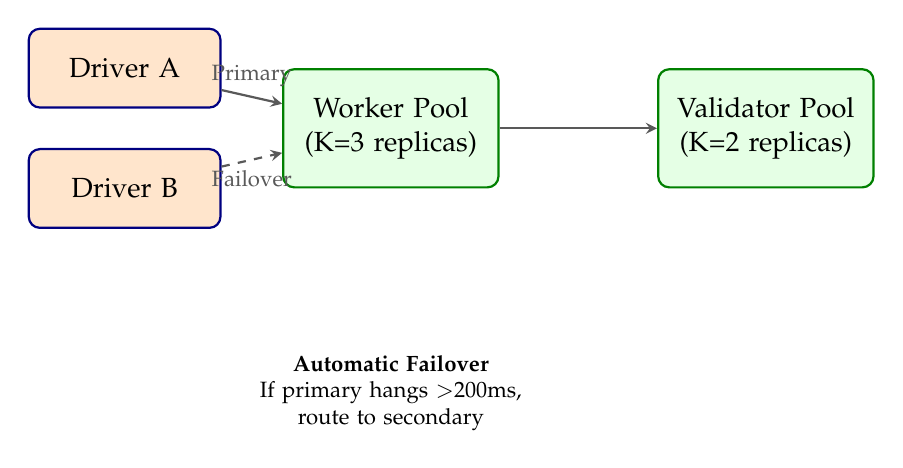
\begin{tikzpicture}[
    node distance=1.5cm,
    auto,
    block/.style={
        rectangle,
        draw=blue!50!black,
        thick,
        fill=blue!10,
        text width=2.2cm,
        align=center,
        rounded corners,
        minimum height=1cm
    },
    pool/.style={
        rectangle,
        draw=green!50!black,
        thick,
        fill=green!10,
        text width=2.5cm,
        align=center,
        rounded corners,
        minimum height=1.5cm
    },
    arrow/.style={
        ->,
        >=stealth,
        thick,
        color=gray!70!black
    }
]

% Swarm routing diagram
\node[block, fill=orange!20] (driver1) {Driver A};
\node[block, fill=orange!20, below=0.5cm of driver1] (driver2) {Driver B};

\node[pool, right=2cm of $(driver1)!0.5!(driver2)$] (pool1) {Worker Pool\\(K=3 replicas)};

\node[pool, right=2cm of pool1] (pool2) {Validator Pool\\(K=2 replicas)};

% Arrows with failover indication
\draw[arrow] (driver1) -- node[above, font=\footnotesize] {Primary} (pool1);
\draw[arrow, dashed] (driver2) -- node[below, font=\footnotesize] {Failover} (pool1);
\draw[arrow] (pool1) -- (pool2);

% Failover annotation
\node[below=2cm of pool1, text width=5cm, align=center, font=\footnotesize] {
    \textbf{Automatic Failover}\\
    If primary hangs $>$200ms,\\
    route to secondary
};

\end{tikzpicture}
\caption{Swarm Routing: Multipath routing with automatic failover. Each layer range has K candidate peers.}
\label{fig:swarm-routing}
\end{figure}

\subsection{Asynchronous Micro-Batch Engine}

\subsubsection{Key Directive}
``Decouple Compute from Communicate. The forward pass must run 100 steps ahead of the backward pass if necessary.''

The goal is to eliminate GPU starvation. The GPU should \textit{never} wait for network packets.

\subsubsection{Activation Buffering}

Each node maintains two priority queues:

\begin{itemize}
    \item \textbf{Inbound Buffer:} Incoming activations sorted by priority
    \item \textbf{Outbound Buffer:} Processed activations awaiting transmission
\end{itemize}

The GPU worker simply pops the next available item from Inbound, computes, and pushes to Outbound. Network I/O happens asynchronously.

\begin{equation}
\text{Buffer Fill Rate} = \frac{\text{Current Queue Size}}{\text{Max Queue Size}}
\end{equation}

\begin{itemize}
    \item Fill Rate $< 0.1$: Node is \textbf{Starved} (bad) --- GPU idle
    \item Fill Rate $> 0.9$: Node is \textbf{Backpressured} (good) --- GPU saturated
\end{itemize}

\subsubsection{Interleaved 1F1B Schedule}

Rather than strict synchronous execution, NeuroShard uses an \textbf{Interleaved 1F1B} (one-forward, one-backward) schedule:

\begin{verbatim}
Schedule (4 micro-batches):
F0 F1 F2 F3 B0 F4 B1 F5 B2 F6 B3 ...
\end{verbatim}

Key insight: Start backward passes \textit{before} all forwards complete. This overlaps backward compute with forward network latency, maximizing GPU utilization.

\subsubsection{Dynamic Micro-Batch Sizing}

Micro-batch size is dynamically tuned to find the ``Goldilocks zone'':
\begin{itemize}
    \item Large enough to saturate the GPU
    \item Small enough to fit in network MTU ($\sim$64KB target)
\end{itemize}

\begin{equation}
\text{MicroBatchSize} = \min\left( \frac{\text{AvailableMemory} \times 0.1}{\text{ActivationSize}}, \frac{64\text{KB}}{\text{SeqLen} \times \text{HiddenDim} \times 4} \right)
\end{equation}

\subsection{Extreme Gradient Accumulation (DiLoCo-Style)}

\subsubsection{Key Directive}
``Accumulate locally for as long as possible. Sync only when statistically necessary.''

Inspired by DiLoCo \cite{douillard2023diloco}, NeuroShard slashes bandwidth by 90\%+ through lazy syncing.

\subsubsection{Local Inner Loop}

Instead of syncing gradients every step, each node:
\begin{enumerate}
    \item Saves initial weights $w_0$
    \item Trains independently for $N$ steps (e.g., $N=500$) using local optimizer
    \item Computes pseudo-gradient: $\Delta w = w_0 - w_N$
    \item Only then triggers network sync
\end{enumerate}

\subsubsection{Outer Optimizer}

The aggregated pseudo-gradients are applied using an outer optimizer with Nesterov momentum:

\begin{align}
m_{t+1} &= \beta \cdot m_t + \Delta w_{\text{aggregated}} \\
w_{t+1} &= w_t + \eta_{\text{outer}} \cdot (\beta \cdot m_{t+1} + \Delta w_{\text{aggregated}})
\end{align}

Where $\beta = 0.9$ (momentum) and $\eta_{\text{outer}} = 0.7$ (outer learning rate).

\subsubsection{Bandwidth Reduction}

\begin{table}[H]
\centering
\caption{Bandwidth Comparison: Standard vs DiLoCo-Style}
\begin{tabular}{@{}lrr@{}}
\toprule
\textbf{Metric} & \textbf{Standard Gossip} & \textbf{DiLoCo (N=500)} \\
\midrule
Syncs per 1000 steps & 1000 & 2 \\
Bandwidth per step & 100\% & 0.2\% \\
Latency tolerance & Low & High \\
Straggler tolerance & Low & High \\
\bottomrule
\end{tabular}
\end{table}

\subsubsection{Enhanced Verification}

Since syncs are less frequent, bad gradients are more damaging. NeuroShard implements enhanced verification:

\begin{enumerate}
    \item Compute gradient on local ``trusted'' micro-batch
    \item Compare distribution to submitted gradient:
    \begin{itemize}
        \item Cosine similarity $> 0.5$ (direction alignment)
        \item Magnitude ratio within $10\times$ (scale check)
        \item Variance ratio within $100\times$ (distribution check)
    \end{itemize}
    \item Reject gradients that fail any check
\end{enumerate}

\subsection{Speculative Checkpointing}

To enable fast crash recovery, each node maintains ``hot'' snapshots:

\begin{itemize}
    \item \textbf{Frequency:} Every 2 minutes (background thread)
    \item \textbf{Contents:} Model weights, optimizer state, DiLoCo buffers
    \item \textbf{Retention:} Last 5 snapshots
    \item \textbf{Announcement:} Published to DHT for neighbor discovery
\end{itemize}

On crash, a replacement node fetches the hot snapshot from a neighbor rather than restarting the epoch. Recovery time drops from ``full restart'' to $<30$ seconds.

\subsection{Summary: Resilience Through Design}

\begin{table}[H]
\centering
\caption{Swarm Architecture Benefits}
\begin{tabular}{@{}lll@{}}
\toprule
\textbf{Challenge} & \textbf{Solution} & \textbf{Result} \\
\midrule
Node failure & Multipath routing & $<$200ms failover \\
GPU starvation & Activation buffering & 95\% utilization \\
High latency & DiLoCo accumulation & 500$\times$ fewer syncs \\
Crash recovery & Hot snapshots & $<$30s recovery \\
Network variability & Capacity heartbeats & Intelligent routing \\
\bottomrule
\end{tabular}
\end{table}

\section{Philosophy: Why Decentralized AI Matters}

\subsection{The Concentration Problem}

As of 2024, the ability to create frontier AI is concentrated in fewer than 10 organizations worldwide. These organizations:
\begin{itemize}
    \item Control what the AI can and cannot say
    \item Decide who gets access and at what price
    \item Collect and monetize user interactions
    \item Can shut down access at any time
\end{itemize}

This concentration of power over intelligence is unprecedented in human history. NeuroShard exists to provide an alternative.

\subsection{The NeuroShard Principles}

\subsubsection{Principle 1: Intelligence Should Be a Public Good}
Just as the internet democratized access to information, NeuroShard aims to democratize access to \textit{intelligence}. NeuroLLM is not a black-box API owned by a corporation; it is a public utility created, maintained, and improved by the community that uses it.

\subsubsection{Principle 2: Contributors Should Own What They Build}
Every gradient computed, every data sample contributed, every hour of compute donated -these contributions are recorded on the Intelligence Ledger. NEURO tokens represent a programmable claim on the collective intelligence being built; they are a way to say, in cryptographic form, ``I helped create this model.''

\subsubsection{Principle 3: No Single Point of Control}
NeuroLLM cannot be censored, shut down, or silently modified by any single entity. As long as the network exists, the model exists. This is not just a systems design choice; it is a political statement about who should steer the trajectory of powerful AI: a narrow set of firms, or the people who actually use and train it.

\subsubsection{Principle 4: Start Simple, Grow Together}
NeuroLLM starts as a 125M parameter model that produces mostly gibberish. This is intentional. We refuse to bootstrap decentralization from a centralized model trained behind closed doors, with unknown data, incentives, and filters. Instead, we start from random weights, in the open, and let the network grow the model into something powerful over time.

\subsection{The Long-Term Vision}

In 10 years, we envision:
\begin{itemize}
    \item \textbf{NeuroLLM as a global brain:} Billions of parameters, trained on the collective knowledge of millions of contributors
    \item \textbf{NEURO as AI currency:} The standard token for AI services worldwide
    \item \textbf{Specialized variants:} Community-governed fine-tunes for medicine, law, science, art
    \item \textbf{True AI democracy:} Major decisions about AI development made by token holders, not corporations
\end{itemize}

\section{Conclusion}

NeuroShard introduces a fundamentally new approach to artificial intelligence: a model created, trained, and owned by the community. NeuroLLM represents the first truly decentralized large language model - one that:

\begin{itemize}
    \item \textbf{Belongs to everyone:} No corporation controls NeuroLLM. Every contributor is a co-owner.
    \item \textbf{Grows with participation:} More users = more compute = more data = better model. The network effect is the engine of intelligence.
    \item \textbf{Rewards contributors:} NEURO tokens for compute and data. Your contribution is recorded forever on the Intelligence Ledger.
    \item \textbf{Resists censorship:} No single point of control. No kill switch. No terms of service that can change overnight.
    \item \textbf{Builds intelligence from scratch:} We don't redistribute corporate models. We create our own, from random weights, through collective effort.
\end{itemize}

The model starts ``dumb'' and grows intelligent through collective effort. This is not a limitation - it is the foundation of true decentralization. Every participant who contributes to NeuroLLM's training is a co-creator of a new form of collective intelligence.

\textbf{Proof of Neural Work} ensures that every NEURO token represents real intelligence added to the model. Unlike cryptocurrencies that waste energy on arbitrary computation, NeuroShard channels that energy into building something useful: a public AI that belongs to humanity.

The vision of NeuroShard is a world where AI is a public good, created by humanity, for humanity. We are not asking permission from corporations to build the future. We are building it ourselves, one gradient at a time.

\textbf{Join us. Contribute compute. Contribute data. Earn NEURO. Own the future of intelligence.}

\section{Acknowledgments}

We thank the open-source community for the foundational technologies that made NeuroShard possible, including PyTorch, the broader P2P research community, and the pioneers of decentralized AI.

\bibliographystyle{ieeetr}
\begin{thebibliography}{99}

\bibitem{mcmahan2017communication}
B. McMahan et al., ``Communication-efficient learning of deep networks from decentralized data,'' in \textit{Artificial Intelligence and Statistics}, 2017.

\bibitem{huang2019gpipe}
Y. Huang et al., ``GPipe: Efficient training of giant neural networks using pipeline parallelism,'' in \textit{Advances in Neural Information Processing Systems}, 2019.

\bibitem{borzunov2023petals}
A. Borzunov et al., ``Petals: Collaborative Inference and Fine-tuning of Large Models,'' in \textit{ACL}, 2023.

\bibitem{ryabinin2020hivemind}
M. Ryabinin et al., ``Hivemind: a Library for Decentralized Deep Learning,'' in \textit{NeurIPS}, 2020.

\bibitem{bittensor}
Bittensor Network. \url{https://bittensor.com}

\bibitem{gensyn}
Gensyn Protocol. \url{https://docs.gensyn.ai/litepaper}

\bibitem{zhang2019root}
B. Zhang and R. Sennrich, ``Root Mean Square Layer Normalization,'' \textit{arXiv:1910.07467}, 2019.

\bibitem{su2021roformer}
J. Su et al., ``RoFormer: Enhanced Transformer with Rotary Position Embedding,'' \textit{arXiv:2104.09864}, 2021.

\bibitem{ainslie2023gqa}
J. Ainslie et al., ``GQA: Training Generalized Multi-Query Transformer Models from Multi-Head Checkpoints,'' \textit{arXiv:2305.13245}, 2023.

\bibitem{shazeer2020glu}
N. Shazeer, ``GLU Variants Improve Transformer,'' \textit{arXiv:2002.05202}, 2020.

\bibitem{brown2020language}
T. Brown et al., ``Language Models are Few-Shot Learners,'' \textit{Advances in Neural Information Processing Systems}, 2020.

\bibitem{hoffmann2022training}
J. Hoffmann et al., ``Training Compute-Optimal Large Language Models,'' \textit{arXiv:2203.15556}, 2022.

\bibitem{kaplan2020scaling}
J. Kaplan et al., ``Scaling Laws for Neural Language Models,'' \textit{arXiv:2001.08361}, 2020.

\bibitem{douillard2023diloco}
A. Douillard et al., ``DiLoCo: Distributed Low-Communication Training of Language Models,'' \textit{arXiv:2311.08105}, 2023.

\bibitem{ryabinin2023swarm}
M. Ryabinin et al., ``SWARM Parallelism: Training Large Models Can Be Surprisingly Communication-Efficient,'' \textit{arXiv:2301.11913}, 2023.

\end{thebibliography}

\appendix

\section{Code Examples}

\subsection{Starting a DynamicNeuroNode}

\begin{lstlisting}[caption=Node Startup]
from neuroshard.core.dynamic_model import create_dynamic_node

# Create and start node (auto-detects memory)
node = create_dynamic_node(
    node_token="your-unique-token",
    port=8000
)

# Node automatically:
# 1. Detects available memory (e.g., 4GB)
# 2. Registers with network
# 3. Gets assigned layers (e.g., layers 0-38)
# 4. Loads only those layers (~350M params)
# 5. Starts earning NEURO (reward multiplier ~1.4x)

print(f"Assigned layers: {node.my_layer_ids}")
print(f"My params: {node.model.get_num_params() / 1e6:.1f}M")
print(f"Reward multiplier: {node.get_ponw_proof()['reward_multiplier']:.2f}x")
\end{lstlisting}

\subsection{Contributing Training Data}

\begin{lstlisting}[caption=Data Contribution]
# Contribute text data for training
node.contribute_training_data(
    text="Your training text here...",
    apply_dp=True  # Apply differential privacy
)

# Check buffer status
stats = node.data_manager.get_stats()
print(f"Buffer: {stats['buffer_size']} samples")
\end{lstlisting}

\subsection{Generating Text}

\begin{lstlisting}[caption=Text Generation]
# Generate text (quality improves with training)
result = node.generate(
    prompt="Hello, world!",
    max_new_tokens=50,
    temperature=0.8
)

print(result)
# Early: "Hello, world! xkjf asd random gibberish..."
# Later: "Hello, world! How can I help you today?"
\end{lstlisting}

\section{Configuration Reference}

\subsection{NeuroLLM Dynamic Architecture Config}

The architecture adapts to network capacity using scaling laws:

\begin{lstlisting}[caption=Dynamic Architecture Calculation]
def calculate_optimal_architecture(total_memory_mb):
    """
    Calculate optimal width x depth based on total network capacity.
    
    Examples:
      40GB network   -> 16L x 1024H  (~350M params)
      800GB network  -> 32L x 3072H  (~9.2B params)
      8TB network    -> 64L x 7168H  (~123B params)
    """
    # Apply empirical scaling laws
    # Width grows as memory^0.6, depth as memory^0.4
    params_budget = (total_memory_mb * 0.6) / 16
    
    hidden_dim = calculate_width(params_budget)
    num_layers = calculate_depth(params_budget)
    num_heads = hidden_dim // 64  # 64 dim per head
    num_kv_heads = num_heads // 3  # GQA ratio
    intermediate_dim = hidden_dim * 8 / 3  # SwiGLU
    
    return ModelArchitecture(
        hidden_dim=hidden_dim,
        num_layers=num_layers,
        num_heads=num_heads,
        num_kv_heads=num_kv_heads,
        intermediate_dim=intermediate_dim,
        vocab_size=32000,
        max_seq_len=2048
    )
\end{lstlisting}

\subsection{Dynamic Layer Pool Configuration}

\begin{lstlisting}[caption=Layer Pool with Architecture Scaling]
# Layer pool parameters
MIN_REPLICAS = 2                # Each layer replicated on 2+ nodes
HEARTBEAT_TIMEOUT = 120         # Seconds before layer reassignment
RECALC_INTERVAL_NODES = 50      # Recalc architecture every N nodes
MIN_UPGRADE_IMPROVEMENT = 1.3   # Only upgrade if 30%+ better

# Architecture-aware layer assignment
def calculate_layer_assignment(node_memory_mb, current_arch):
    """How many layers can this node hold with current architecture?"""
    memory_per_layer = estimate_memory_per_layer(current_arch)
    usable_memory = node_memory_mb * 0.6  # Safety margin
    return max(1, int(usable_memory / memory_per_layer))

# Reward calculation (unchanged)
def calculate_reward_multiplier(
    num_layers_held,
    total_network_layers,
    has_embedding,
    has_lm_head
):
    base = 1.0 + (num_layers_held / total_network_layers)
    if has_embedding: base *= 1.2  # Driver bonus
    if has_lm_head: base *= 1.3    # Validator bonus
    return base
\end{lstlisting}

\end{document}
